\chapter{Arquitectura de Aplicaciones SaaS}
La arquitectura de software describe como están conectados los subsistemas que componen un software, para alcanzar los requerimientos funcionales y no funcionales de la aplicación \cite{Fox2013-ct}.

\section{Patrones de Diseño SaaS} 
Dado el concepto de patrón de diseño:
\begin{displayquote}
Los patrones de diseño son estructuras reutilizables, comportamientos, estrategias o técnicas que contienen una solución demostrada para un conjunto de problemas similares, separando las cosas que son dinámicas de las estáticas.
\cite{Fox2013-ct}
\end{displayquote}
    
    Los patrones de diseño permiten generalizar la experiencia de muchos años de programación en soluciones que sirven para encarar una conjunto de soluciones. 
    En las aplicaciones SaaS, algunos de los patrones de diseño que se utilizan son:
\begin{itemize}
    \item Cliente-Servidor
    \item Arquitectura en tres capas
    \item Modelo-Vista-Controlador
    \item Active Record
    \item Template View
    \item Principio REST
\end{itemize}


    \begin{figure}[H]
        \centering
        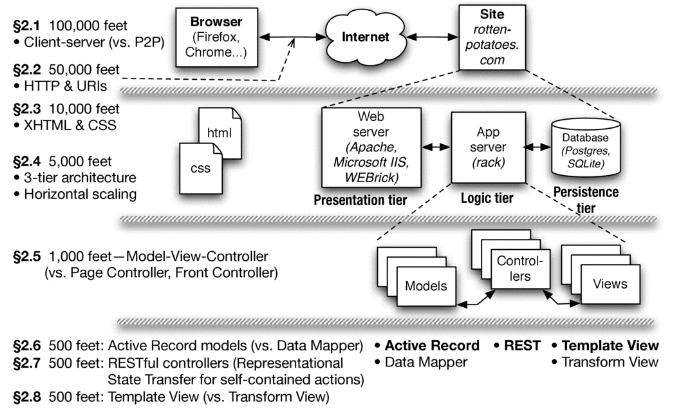
\includegraphics[width=0.85\textwidth]{saas-arch}
        \caption{Estructuras en distintos niveles en una arquitectura SaaS \protect\cite{Fox2013-ct}}
        \label{fig:saas-arch}
    \end{figure}

En la figura \ref{fig:saas-arch} se observan la estructura de una arquitectura SaaS por niveles y los patrones de diseño que se aplican en cada uno. Estos patrones se describen en las secciones subsiguientes.
\subsection{Arquitectura Cliente-Servidor}
    
En la arquitectura cliente-servidor, lo estático es la separación de responsabilidades entre el cliente y el servidor, independiente de la implementación de ambos. Un cliente (navegador web) se encarga interactuar de con el usuario y de enviar pedidos al servidor; y, un servidor responde a los pedidos de muchos clientes. 
\subsection{Arquitectura de 3 Niveles y Escalabilidad Horizontal}

Una aplicacion SaaS suele dividirse tres capas lógicas:
\begin{itemize}
    \item Capa de Presentación
    \item Capa Lógica
    \item Capa de Datos
\end{itemize}
\begin{figure}[H]
        \centering
        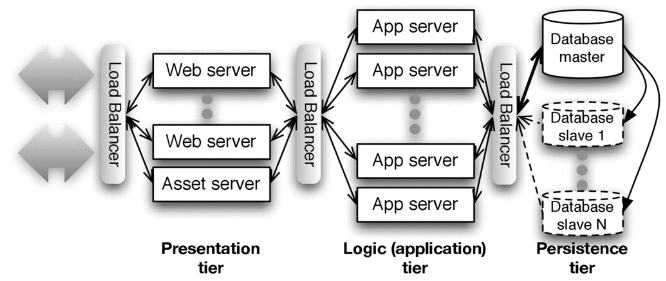
\includegraphics[width=0.90\textwidth]{three-tier-arch}
        \caption{Arquitectura en tres capas \protect\cite{Fox2013-ct}}
        \label{fig:three-tier-arch}
    \end{figure}
La capa de presentación consiste usualmente de un servidor web que acepta pedidos de los usuarios y los reenvía a la capa lógica para retornar las vistas que conforman la interfaz de usuario. Luego, la capa lógica se ejecuta en un servidor de aplicación, que es donde se genera el contenido dinámico. Finalmente, la capa de persistencia consiste en una base de datos que contiene la información de la aplicación. En esta arquitectura, como muestra la figura \ref{fig:three-tier-arch}, las entidades dentro de una capa no se comunican entre ellos, lo que permite escalar los recursos para satisfacer variaciones de demanda con tecnologías de Cloud Computing.

\subsection{Arquitectura Modelo-Vista-Controlador}

\begin{figure}[H]
        \centering
        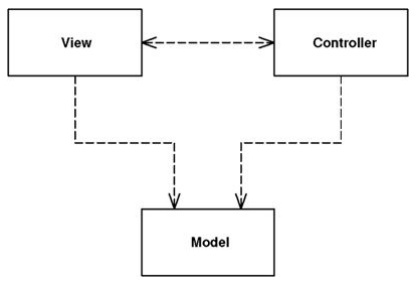
\includegraphics[width=0.55\textwidth]{mvc-arch}
        \caption{Patron de Arquitectura MVC \protect\cite{Fowler2012-az}}
        \label{fig:mvc-arch}
    \end{figure}

El patrón Modelo-Vista-Controlador (MVC) es un patrón de arquitectura que organiza el código de una aplicación en tres tipos \cite{Fox2013-ct}:  
\begin{itemize}
    \item Los modelos se encargan de los datos manipulados por la aplicación (como almacenar, operar y cambiar los datos).
    \item Las vistas muestran información acerca de los modelos y son la interfaz entre el usuario y los datos. 
    \item Los controladores actúan de intercomunicadores entre las vistas y los modelos. Cada controlador corresponde a un modelo, y define que acciones (solicitudes HTTP) corresponden a que método del modelo. De igual manera, sintetiza las vistas que son enviadas a la capa de presentación.
\end{itemize}

\subsection{Active Record}
\begin{figure}[H]
        \centering
        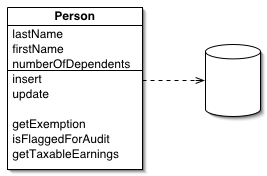
\includegraphics[width=0.55\textwidth]{active-record}
        \caption{Patron de Arquitectura MVC \protect\cite{Fowler2012-az}}
        \label{fig:active-record}
    \end{figure}
\begin{displayquote}
"Un objeto que envuelve una fila en una tabla o vista de una base de datos, encapsula el acceso a la base de datos y agrega lógica del negocio sobre esos datos. "
\cite{Fowler2012-az}
\end{displayquote}
Active Record es un patrón de diseño para el manejo de base de datos. Permite que una clase sea capaz de crear, modificar, leer y eliminar (en inglés, CRUD) instancias de si misma en una base de datos, dado que una instancia de un objeto de la clase corresponde a una fila de la tabla de la base de datos.

\subsection{Routeo mediante REST}

Los controladores son los encargados de mapear las solicitudes HTTP al correspondiente metodo en el modelo. Este mapeo se llama rutas o routeo. Las solicitudes HTTP estan compuestas de su URI y de su método HTTP. En su tesis doctoral, \citeA{Fielding-rt} propuso una manera de describir en las solicitudes HTTP las acciones que se desea ejecutar y sobre que recursos.

\begin{figure}[H]
        \centering
        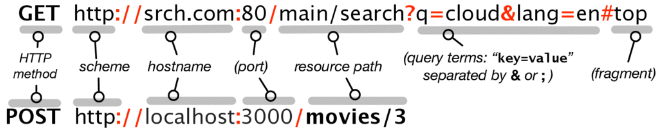
\includegraphics[width=0.85\textwidth]{http-request}
        \caption{Solicitud HTTP \protect\cite{Fox2013-ct}}
        \label{fig:http-request}
\end{figure}

La Transferencia de Estado Representacional (REST) es una de las maneras en que los navegadores web pueden realizar transacciones a través de HTTP. REST simplifica la integración de servicios SaaS, siendo utilizado para la construcción de APIs para exponer los servicios en una Arquitectura Orientada a Servicios, donde la comunicación entre ellos es independiente (en ingles, self-contained) de una sesión.

Las APIs RESTful son utilizadas por muchos sitios, incluyendo Google 
\cite{Google-Inc2016-lm}, Amazon \cite{Aws2016-iu}, Twitter \cite{Twitter2016-df} y LinkedIn \cite{LinkedIn2016-am}.

Una API RESTful es una interfaz de aplicación web (API) que utiliza HTTP para hacer las pedidos de datos GET, POST, PUT y DELETE; y, descompone una transacción en módulos, cada uno de los cuales se encarga de una parte de la operación. Se utiliza la pedido PUT para cambiar el estado o actualizar un recurso, GET para obtener un recurso, POST para crear un recurso y DELETE para removerlo. Actualmente los modelos REST de Amazon Simple Storage Service (S3) \cite{Aws2016-tc}, Openstack Swift \cite{OpenStack2016-ht} y Cloud Data Management Interface (CDMI) \cite{Snia2016-vq} son los más populares \cite{Richardson2008-ng}.

\subsection{Vista de Plantillas (Template View)}

\begin{figure}[H]
        \centering
        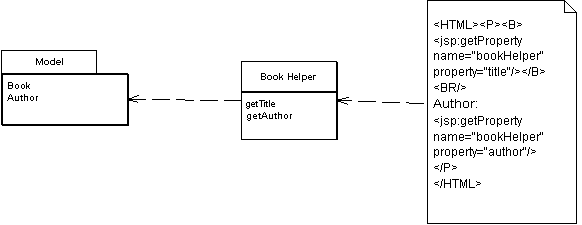
\includegraphics[width=0.90\textwidth]{template-view}
        \caption{Template View \protect\cite{Fowler2012-az}}
        \label{fig:template-view}
    \end{figure}

Este patrón permite la creación de paginas web en base a plantillas que incluyen contenido de variables que luego son substituidas para generar contenido estatico (HTML) que es enviado al navegador web del usuario final. 
De acuerdo con MVC, las vistas deben contener la minima cantidad de codigo posible.

\section{Frameworks SaaS}
En un principio, cada página web era programada a mano: actualizar un sitio web significaba editar HTML y un rediseño implicaba rehacer cada página, una por una. Con el tiempo, los sitios web crecieron y se volvieron más “ambiciosos” por lo que este proceso se volvió tedioso, consumía tiempo y era inmantenible.

Un grupo de programadores en la NCSA (Centro Nacional de Aplicaciones de Supercomputación, donde Mosaic, el primer navegador web gráfico fue desarrollado), resolvieron este problema permitiendo que el servidor web se conecte con programas externos que dinámicamente generaban HTML. Este protocolo se llamó Interfaz de Entrada Común (CGI o Common Gateway Interface, con lo cual las páginas web eran generadas “a pedido” dinámicamente. 

Sin embargo, CGI presentó problemas debido a que los scripts en CGI tienen que incluir varias plantillas repetitivas que no permiten reutilizar mucho código y tienen una curva de aprendizaje empinada.

En este sentido, se desarrollaron los frameworks de desarrollo web que proveen una infraestructura para la programación de aplicaciones, de manera que el programador pueda escribir código mantenible sin tener que re-inventar la rueda. \cite{Holovaty2016-nm}


\subsection{Laravel}
Laravel es un framework de desarrollo web open-source escrito en PHP que sigue una arquitectura Modelo-Vista-Controlador, que refuerza la separación de la logica del negocio de la lógica de presentación asociada a la interfaz de usuario. Laravel soporta transacciones RESTful, plantillas, JSON APIs y gestión de paquetes con Composer \cite{Bean2015-zt}. Laravel fue reportado ser el Framework de desarrollo web para PHP más popular en 2015 \cite{SitePoint2015-yl}.

Laravel utiliza una máquina virtual basada en Vagrant, llamada Homestead, que maneja y configura el ambiente de desarrollo. La virtualización consiste en utilizar una máquina virtual para correr un servidor web, una base de datos y scripts; es decir, desarrollar aplicaciones y sitios web dinámicos. Se pueden crear múltiples máquinas virtuales para varios proyectos, las cuales también pueden ser borradas cuando no se necesiten sin afectar al resto.  De igual manera, pueden ser re-creadas en poco tiempo \cite{Wu2016-ws}. Un sitio que vale la pena mencionar es \citeA{Tumblr2016-mn}, que experimentó drásticos mejoras de desempeño al migrar a PHP 7. 

\subsection{Django}
Django es un framework de desarrollo web open-source escrito en Python, que sigue la arquitectura Modelo-Vista-Plantilla. El principal objetivo de Django es facilitar la creación de sitios web complejos. Enfatiza la reusabilidad y la capacidad de “enchufar” componentes, desarrollo rápido y el principio de DRY (en  inglés, Don’t Repeat Yourself) \cite{Holovaty2009-jr}. Algunos sitios web desarrollados con Django son:
\begin{itemize}
    \item Disqus \cite{Robenolt2013-cb}
    \item \citeA{Instagram2016-cp}
    \item Bitbucket \cite{Django2012-bt}
    \item \citeA{OpenStack2016-vh}
\end{itemize}

\subsection{Ruby on Rails}
Ruby on Rails es un framework de desarrollo web escrito en Ruby, cuya filosofía incluye dos principios principales: DRY (Don’t Repeat Yourself) y Convention Over Configuration (convención sobre configuración) que implica minimizar el número de decisiones que un desarrollador necesita tomar (configuración), ganando así en simplicidad pero no perdiendo flexibilidad por ello.
Algunos sitios web desarrollados con Ruby on Rails son:
\begin{itemize}
    \item 500px \cite{Liu2015-dx}
    \item Airbnb \cite{Weksler2015-ip}
    \item \citeA{GitHub2009-gt}
    \item \citeA{Bloomberg2012-ue}
\end{itemize}
